\section{Implementation}

\subsection{General Structure}
\label{sub:genstruct}

We implemented the STRIPS algorithm in a way that it can generically be used for different problems. Based on this structure we implemented the specific problem and a domain specific heuristic.

Figure \ref{fig:uml1} visualizes the following explanations in a UML class diagram. A larger image of this diagram is attached to this report (see appendix \ref{app:included}).

\begin{figure}[hbt]
  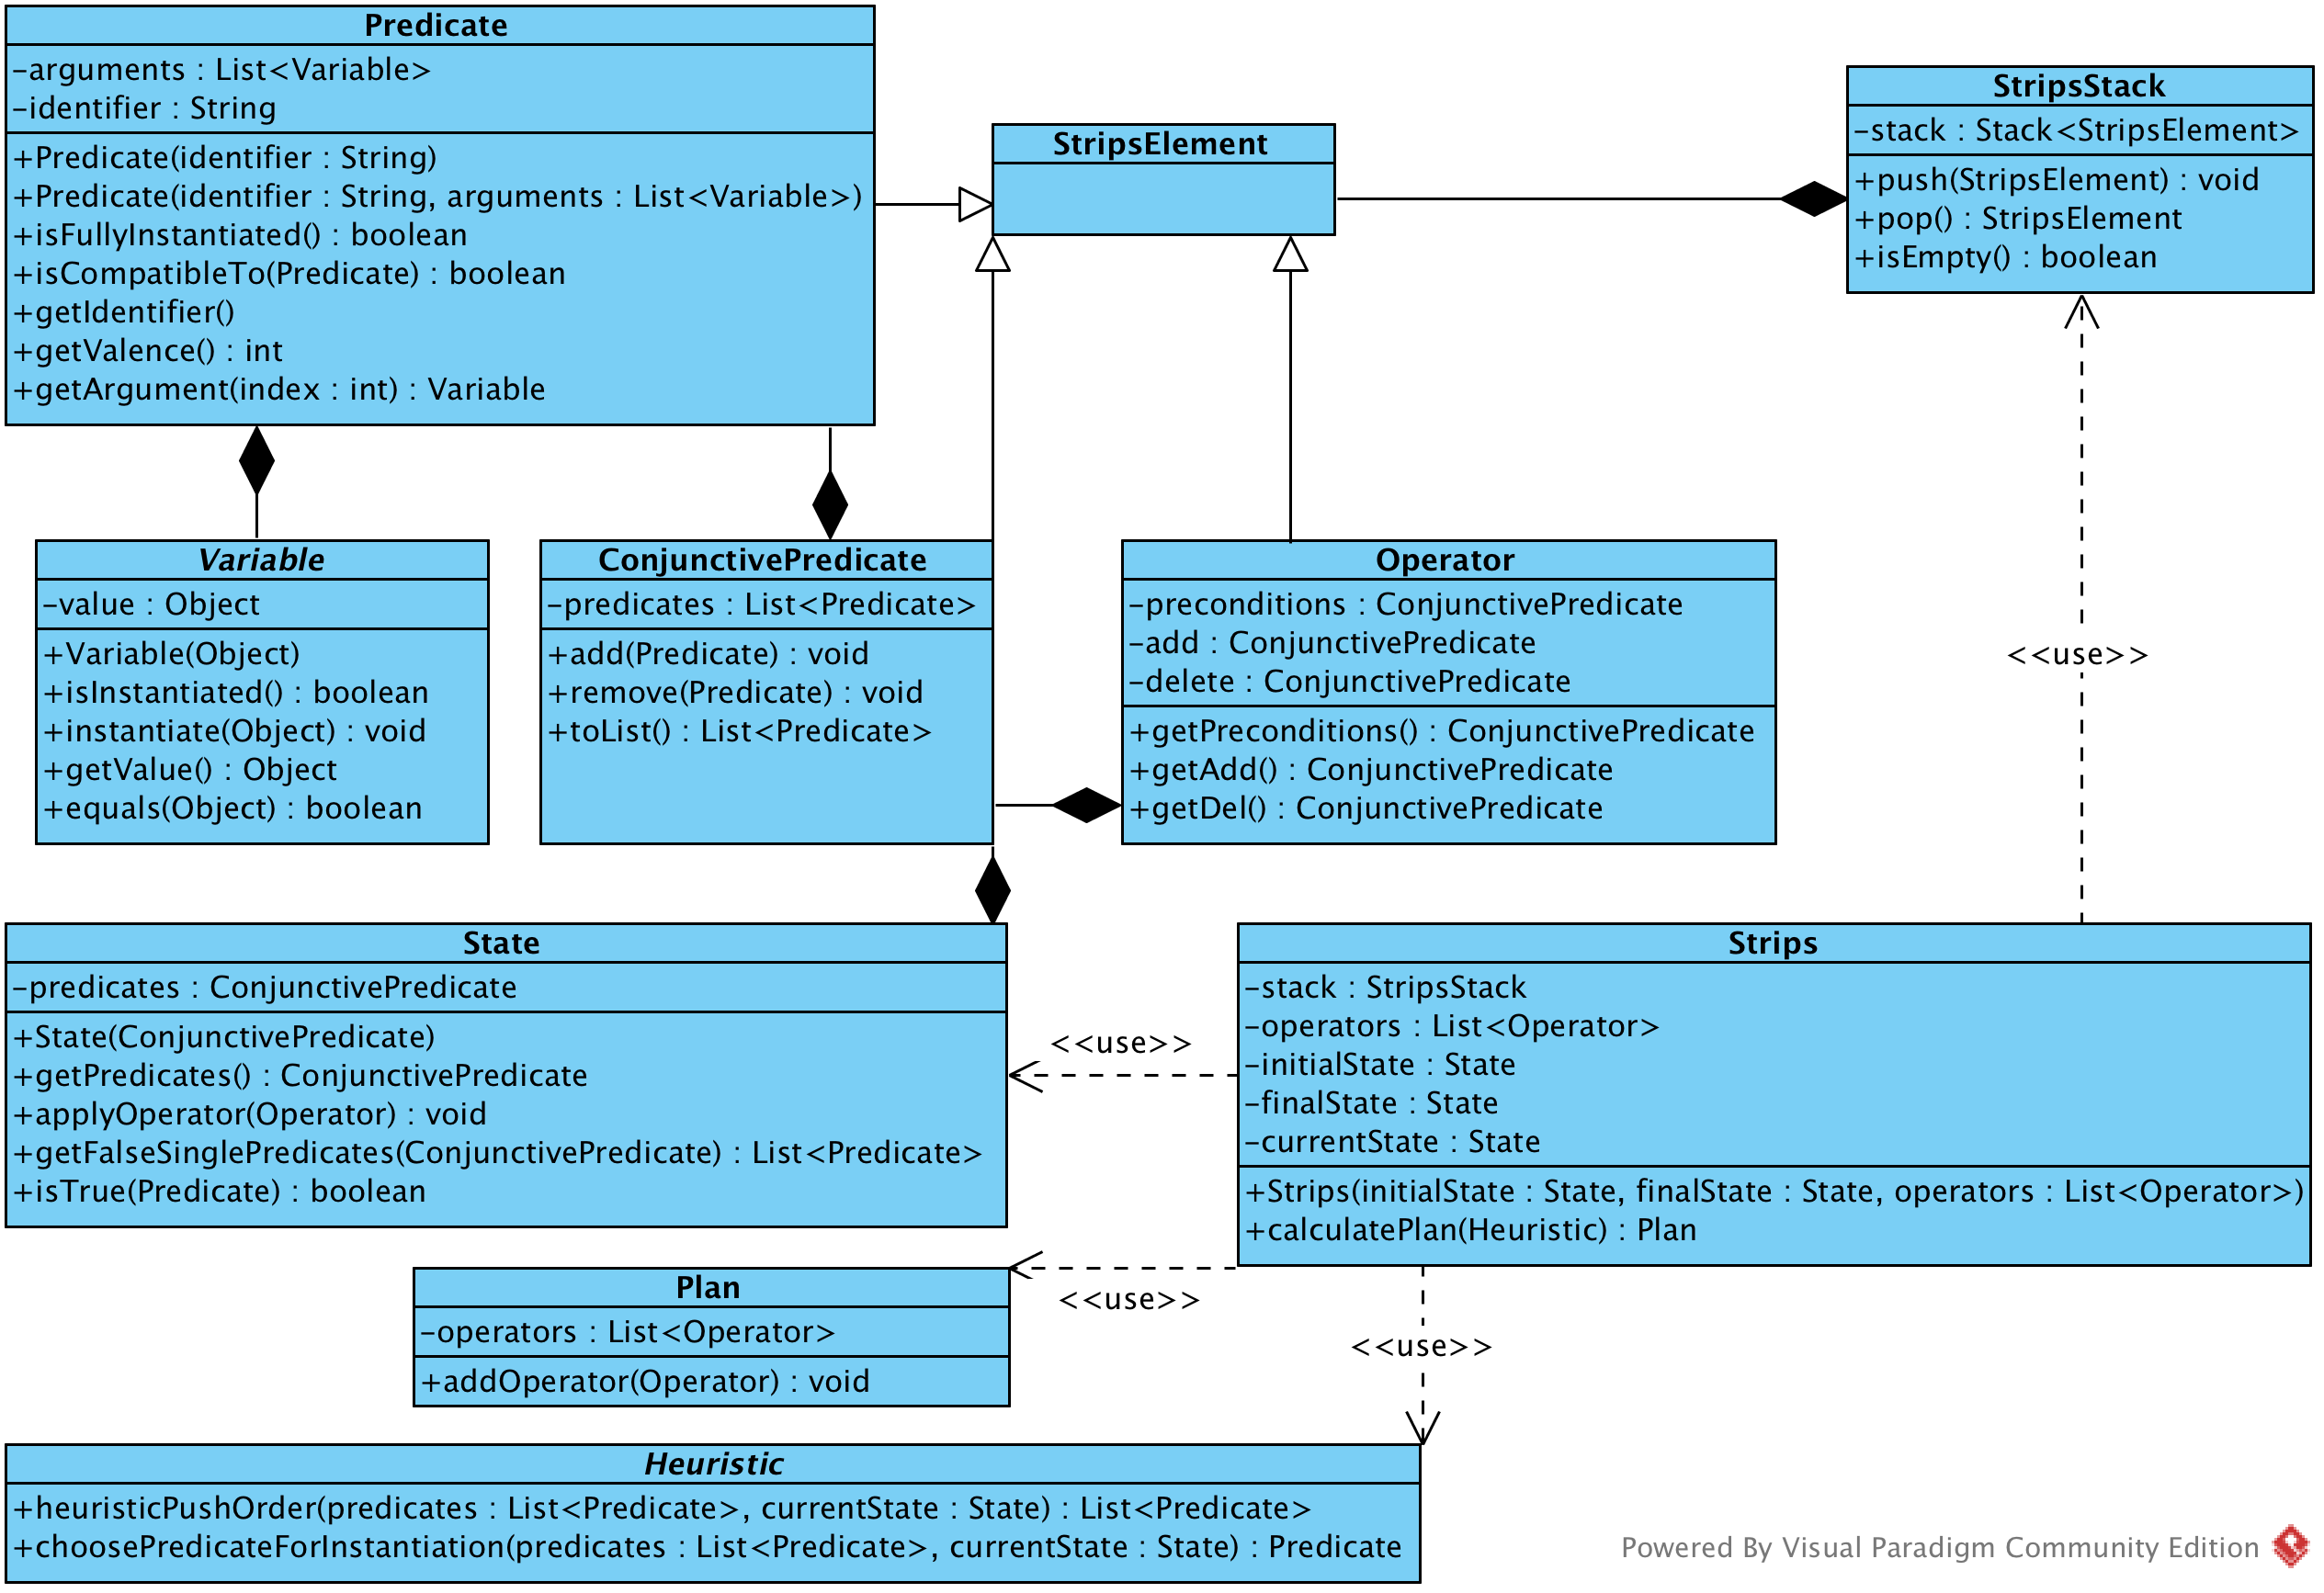
\includegraphics[width=1.1\textwidth]{uml/CD1}
  \caption{UML Class Diagram of STRIPS classes}
  \label{fig:uml1}
\end{figure}

The implementation is centered around the \texttt{Strips} class. Objects of this class use a \texttt{StripsStack} to solve a specific problem, given \textit{initialState} and \textit{finalState} of class \texttt{State} and a list of \texttt{Operator} objects. The method \textit{calculatePlan} takes a realization of the abstract class \texttt{Heuristic} and calculates a \texttt{Plan} object based on the STRIPS algorithm and the domain specific heuristics specified in the \textit{heuristic}. 

The stack provided by \texttt{StripsStack} can be filled with objects of the class \texttt{StripsElement}, which is the superclass for \texttt{Predicate}, \texttt{Operator}, and \texttt{ConjunctivePredicate}. 

\texttt{Predicate} objects have an unique \textit{identifier} and a list of \texttt{Variable} objects that represent the arguments of the predicate. \texttt{Variable} objects can take another \texttt{Object} as their \textit{value} or have a \textit{value} of \texttt{null} if the argument is not instantiated. 

Objects of \texttt{ConjunctivePredicate} represent a list of single \texttt{Predicate} objects. They are used in other classes such as \texttt{State} or \texttt{Operator} to handle conjunction lists of predicates.

The \texttt{Operator} class represents operators in the STRIPS algorithm with their lists of preconditions and the postconditions split up in both a \texttt{ConjunctivePredicate} \textit{add} and \textit{delete}.


\subsection{Problem Implementation}

It should be noted that none of the classes introduced in the previous subsection \ref{sub:genstruct} are implementations of a specific domain dependent problem - they are a general representation of the STRIPS algorithm that works for a large set of problems.

% TODO: implementation of coffee problem

\subsection{Heuristic Details}

In this section we present some chosen details of our implementation that we consider more relevant. We focus on demonstrating the implementation of the heuristics explained in subsection \ref{subsub:heuristics}. To get a full understanding of the code one might want to look at the complete source code attached to this report (see Appendix \ref{app:included}).

The most important heuristic in terms of step minimization is choosing the best coffee machine out of several available ones when instantiating a Machine($o, n$) predicate. Listing \ref{code:instantiate} shows how the STRIPS algorithm finds all possible instantiations of a predicate \textit{singlePred} in the current state. All possible instantiation candidates are then passed to the heuristic, that decides which Machine($o, n$) predicate to choose. 

\begin{lstlisting}[language=Java, 
	caption=Strips method  \textit{instantiate}, 
	keywordstyle=\color{blue},
	stringstyle=\color{red},
	commentstyle=\color{magenta},
	label = {code:instantiate}]
private void instantiate(Predicate singlePred, Heuristic heuristic) {
  List<Predicate> compatiblePredicates = new ArrayList<>();
  for (Predicate currPred : this.currentState.getPredicates().toList()) {
    // find all compatible predicates in current state:
    if (currPred.isCompatibleTo(singlePred)) {
      compatiblePredicates.add(currPred);
    }
  }
  ... 
  // Heuristic chooses one candidate from compatiblePredicates
  Predicate chosenPred = heuristic.choosePredicateForInstantiation(
				compatiblePredicates, currentState);
				
  // instantiate with singlePred with constants of chosenPred
  for (int i = 0; i < chosenPred.getValence(); i++) {
    if (!singlePred.getArgument(i).isInstantiated()) {
      // Update the Java object of the variable.
      // All references to this variable in other predicates
      // will now reference to the instantiated variable.
      singlePred.getArgument(i).instantiate(
                   chosenPred.getArgument(i).getValue());
    }
  } 
}
\end{lstlisting}

In listing \ref{code:machHeur} we can see, how the heuristic chooses a good machine based on the current location of the robot and the next petition he is trying to serve. Each time a new petition is instantiated (based on a Served($o$) predicate), the heuristic object saves the location of this petition in a local variable \textit{lastPetition}. When the heuristic encounters a list of several Machine($o, n$) predicates as candidates to instantiate a single predicate, it will choose the machine with the smallest sum of the distance between the current position and the machine plus the distance between the machine and the next position. This makes sure that a machine is picked that leads to the least possible increase in steps.
\begin{lstlisting}[language=Java, 
	caption=CoffeeHeuristic method  \textit{choosePredicateForInstantiation}, 
	keywordstyle=\color{blue},
	stringstyle=\color{red},
	commentstyle=\color{magenta},
	label = {code:machHeur}]
public Predicate choosePredicateForInstantiation(
  List<Predicate> compatiblePredicates, State currentState) {

  // Save the last instantiated petition to be included in the 
  //distance calculation:
  List<Ppetition> petitionsPred = new ArrayList<>();
  for (Predicate pred : compatiblePredicates) {
    if (pred.getIdentifier().equals(Ppetition.ID)) {
      petitionsPred.add((Ppetition) pred);
    }
  }
  if (!petitionsPred.isEmpty()) {
    lastPetition = petitionsPred.get(0);
  }
  
  // filter out Machine predicates
  List<Pmachine> machinePreds = new ArrayList<>();
  for (Predicate pred : compatiblePredicates) {
    if (pred.getIdentifier().equals(Pmachine.ID)) {
      machinePreds.add((Pmachine) pred);
    }
  }
  
  if (machinePreds.size() > 0) {
    // Find current position in current state:
    Location currentPos = null;
    for (Predicate pred : currentState.getPredicates().toList()) {
      if (pred.getIdentifier().equals(ProbotLocation.ID)) {
        currentPos = (Location) pred.getArgument(0);
        break;
      }
    }
    
    // Find best machine:
    Pmachine closestMachine = null;
    int bestDistanceSoFar = Integer.MAX_VALUE;
    for (Pmachine pred : machinePreds) {
      // distance = distance from current position to machine +
      // distance from machine to last petition
      int distance = Location.distance(currentPos, pred.getLocation(), 
                     lastPetition.getLocation());
	  if (distance < bestDistanceSoFar) {
	    closestMachine = pred;
	    bestDistanceSoFar = distance;
	  }
    }
    return closestMachine;
  }
  ...
}
\end{lstlisting}







